\documentclass[conference,a4paper]{IEEEtran}
\ifdefined\pdfminorversion\pdfminorversion=6\fi
\IEEEoverridecommandlockouts

\usepackage{cite}
\usepackage{amsmath,amssymb,amsfonts}
\usepackage{graphicx}
\usepackage{textcomp}
\usepackage{booktabs}
\usepackage{multirow}
\usepackage{array}
\usepackage[table]{xcolor}
\usepackage{pifont}
\usepackage{hyperref}
\usepackage{listings}
\usepackage{balance}
\usepackage{tikz}
\usepackage{pgfplots}
\usepackage{microtype}
\pgfplotsset{compat=1.18}
\usetikzlibrary{shapes.geometric, arrows.meta, positioning, calc, fit, backgrounds}

% Compact float separation
\setlength{\textfloatsep}{7pt plus 1pt minus 1pt}
\setlength{\floatsep}{6pt plus 1pt minus 1pt}
\setlength{\intextsep}{6pt plus 1pt minus 1pt}
\setlength{\abovecaptionskip}{4pt plus 1pt minus 1pt}
\setlength{\belowcaptionskip}{3pt plus 1pt minus 1pt}

\definecolor{checkgreen}{HTML}{2E7D32}
\definecolor{crossred}{HTML}{C62828}
\definecolor{ourgreen}{HTML}{E8F5E9}
\definecolor{headergray}{HTML}{ECEFF1}
\definecolor{accentblue}{HTML}{1565C0}
\definecolor{boxgray}{HTML}{F8F9FA}

% Publication palette for charts
\definecolor{color_symcode}{HTML}{3867D6}
\definecolor{color_symplan}{HTML}{10AC84}
\definecolor{color_plan}{HTML}{FA8231}
\definecolor{color_contract}{HTML}{8854D0}
\definecolor{chart_grid}{HTML}{E2E8F0}
\definecolor{chart_text}{HTML}{2D3748}
\newcommand{\cmark}{\textcolor{checkgreen}{\ding{51}}}
\newcommand{\xmark}{\textcolor{crossred}{\ding{55}}}

\lstdefinestyle{promptstyle}{
  basicstyle=\ttfamily\scriptsize,
  backgroundcolor=\color{boxgray},
  frame=single,
  rulecolor=\color{black!30},
  breaklines=true,
  columns=fullflexible,
  keepspaces=true,
  xleftmargin=1.5mm,
  xrightmargin=1.5mm,
  aboveskip=3.5pt,
  belowskip=3.5pt
}

\begin{document}

\title{SymPlan: Enhancing Neurosymbolic Mathematical Reasoning in SLMs via Representation and Planning}

\author{
Tay Bui\textsuperscript{1,2},
Huy N. G. Pham\textsuperscript{1,2},
Nhan Ha Le Thanh\textsuperscript{3}\\
\textsuperscript{1} University of Information Technology, Ho Chi Minh City, Vietnam\\
\textsuperscript{2} Vietnam National University, Ho Chi Minh City, Vietnam\\
\textsuperscript{3} FPT University, Ho Chi Minh City, Vietnam\\
\texttt{\small \{24521589, 24520690\}@gm.uit.edu.vn},
\texttt{\small hnhan5355@gmail.com}
}

\maketitle

\begin{abstract}
Mathematical reasoning with language models increasingly relies on executable symbolic programs, yet monolithic program synthesis---which asks a model to simultaneously parse linguistic problem descriptions, formulate algebraic solution plans, and write formal code in a single prompt---imposes an excessive cognitive load on compact small language models (SLMs, $\le 8\text{B}$ parameters). While monolithic methods such as SymCode succeed on frontier architectures, compact backbones under resource-constrained settings (e.g., 4-bit quantization) frequently suffer from semantic misformulation, domain boundary omission, and silent regressions during repair. We introduce SymPlan, an inspectable neurosymbolic framework specifically tailored to provide structural scaffolding for compact models. SymPlan decouples problem solving into three coordinated, contract-governed phases: (1) a \textit{Fused Target-Planning Phase} extracting an explicit target specification, an output type contract, and an algorithmic SymPy roadmap in a single bounded inference step ($\le 256$ tokens); (2) \textit{Contract-Guided SymPy Generation} guiding deterministic code synthesis to satisfy domain invariants and exact arithmetic; and (3) \textit{Targeted Debugging with Anti-Regression Selection}, which couples AST static diagnostics with a lexicographic ranking heuristic to prevent valid intermediate predictions from being overwritten by later repair iterations. Evaluated across six diverse open-weight SLMs (3B to 8B) on the full MATH-500 benchmark under 4-bit quantization, SymPlan consistently outperforms monolithic SymCode by $+3.60\%$ to $+5.20\%$ (averaging $+4.20\%$) and Chain-of-Thought by $+12.64\%$, while improving Execution Success Rate to $89.90\%$ ($+6.07\%$), all without parameter fine-tuning.
\end{abstract}

\begin{IEEEkeywords}
Neurosymbolic Reasoning, Mathematical Problem Solving, Small Language Models, SymPy Code Generation, Algorithmic Planning.
\end{IEEEkeywords}

\section{Introduction}

Large Language Models (LLMs) have achieved remarkable success in multi-step reasoning through Chain-of-Thought (CoT) prompting~\cite{wei2022cot} and structured search~\cite{wang2023selfconsistency,zhou2023leasttomost,wang2023plan}. However, pure autoregressive derivation remains inherently susceptible to arithmetic errors, missing steps, and unfaithful derivations that are difficult to inspect or verify~\cite{lyu2023faithful,he2024olympiadbench}. Program-aided approaches address this deficit by offloading calculation to deterministic interpreters: PAL~\cite{gao2023pal} and PoT~\cite{chen2022pot} delegate numerical operations to Python, while MathCoder~\cite{wang2024mathcoder} and ToRA~\cite{gou2024tora} interleave tool usage with natural-language rationales. More recently, SymCode~\cite{nezhad2025symcode} incorporates the SymPy library~\cite{meurer2017sympy} to support exact symbolic manipulations, equation solving, and modular arithmetic beyond standard floating-point execution.

\begin{figure*}[t]
\centering

\includegraphics[width=0.92\textwidth,height=4.6cm,keepaspectratio]{pipeline-symplan.png}
\caption{Overview of SymPlan. A natural-language problem is first translated into a structured target contract and an ordered symbolic plan before code synthesis. The generated SymPy script is executed in an isolated sandbox; errors trigger AST diagnostics and targeted repair, while the anti-regression selector identifies the optimal execution record.}
\label{fig:overview}
\end{figure*}

Despite these advances, program execution alone does not guarantee correct mathematical interpretation. Translation-based neurosymbolic systems fundamentally depend on the fidelity of the generated program before the solver executes~\cite{lyu2023faithful,pan2023logiclm}. Existing program-aided methods typically couple problem interpretation, solution reasoning, and code synthesis into a monolithic generation step~\cite{gao2023pal,nezhad2025symcode}. While frontier models possess sufficient parameter capacity to manage this joint burden, compact small language models ($\le 8\text{B}$ parameters) struggle severely under monolithic generation. Evaluating six compact open-weight models across MATH-500~\cite{lightman2024verify,hendrycks2021math} under 4-bit quantization~\cite{dettmers2023qlora} reveals four recurrent failure patterns:
\begin{enumerate}
    \item \textit{Semantic misformulation:} runnable code computes an unprompted, distorted, or oversimplified quantity;
    \item \textit{Target contract violation:} code emits an element list when an integer count is queried, or floating-point decimals instead of exact simplified rationals;
    \item \textit{Domain constraint omission:} extraneous or out-of-domain roots are accepted without boundary checks;
    \item \textit{Silent repair regression:} iterative self-debugging yields a runnable script that accidentally overwrites a previously correct answer with an invalid prediction.
\end{enumerate}

To overcome these bottlenecks, we introduce \textbf{SymPlan}, an inspectable neurosymbolic framework designed specifically to provide the structural scaffolding required by compact language models. Rather than relying on unconstrained generation, SymPlan introduces three coordinated stages that match the processing capacity of SLMs:
First, a \textit{Fused Target-Planning Phase} extracts an explicit target specification, an output type contract, and an algorithmic roadmap in a single bounded forward pass ($\le 256$ tokens), preventing multi-turn context drift.
Second, a \textit{Contract-Guided Code Generator} translates this specification into a self-contained SymPy program enforcing exact arithmetic and domain filters.
Third, a \textit{Targeted Debugging Loop} combines interpreter tracebacks and AST static diagnostics with an \textit{Anti-Regression Selection} heuristic that evaluates all execution attempts to conservatively retain the strongest verified candidate.

Our contributions are threefold:
\begin{enumerate}
    \item We empirically characterize the formulation, contract, and debugging failure modes of monolithic symbolic reasoning across six compact models (3B--8B) on the full MATH-500 benchmark.
    \item We propose SymPlan, an open-source neurosymbolic framework combining fused target planning, contract-governed SymPy code synthesis, and anti-regression attempt ranking.
    \item Across six diverse open-weight backbones under 4-bit quantization, SymPlan achieves universal accuracy gains of $+3.60\%$ to $+5.20\%$ (averaging $+4.20\%$) over monolithic SymCode and $+12.64\%$ over CoT, with a $+6.07\%$ increase in Execution Success Rate ($89.90\%$), all without parameter updates.
\end{enumerate}

\section{Related Work}

\textbf{Program-Aided and Symbolic Reasoning.} Program-aided methods use executable code as an intermediate representation, offloading calculation to interpreters. PAL~\cite{gao2023pal} and PoT~\cite{chen2022pot} delegate numerical tasks to Python scripts, while MathCoder~\cite{wang2024mathcoder} and ToRA~\cite{gou2024tora} combine natural-language rationales with tool use. SymCode~\cite{nezhad2025symcode} utilizes SymPy~\cite{meurer2017sympy} for exact algebraic manipulation, calculus, and modular arithmetic. However, monolithic program generation overburdens compact models: if the model misinterprets equations or omits boundary conditions, the interpreter may return successful executions for mathematically invalid answers.

\textbf{Neurosymbolic Formalization and Repair.} Neurosymbolic pipelines translate natural language into formal representations for deterministic execution. Faithful CoT~\cite{lyu2023faithful} separates reasoning from computation, and Logic-LM~\cite{pan2023logiclm} refines symbolic formulations via solver feedback. For code repair, Self-Debugging~\cite{chen2024selfdebug} and Self-Refine~\cite{madaan2023selfrefine} iteratively revise code using error messages. Yet on compact models, unanchored self-debugging frequently induces code cycling or silent regressions. SymPlan provides structural grounding: the frozen target contract anchors intent, while execution history prevents regressive overwrites.

\textbf{Planning in Compact Language Models.} Structured prompting enhances reasoning in compact models. Self-consistency~\cite{wang2023selfconsistency}, Least-to-Most prompting~\cite{zhou2023leasttomost}, Decomposed Prompting~\cite{khot2023decomposed}, and Plan-and-Solve~\cite{wang2023plan} structure problem decomposition. Specialized models such as DeepSeekMath~\cite{shao2024deepseekmath} and Qwen2.5-Math~\cite{yang2024qwen25math}, as well as compact architectures like Phi-3~\cite{abdin2024phi3}, show strong reasoning capabilities with structured guidance. SymPlan bridges these directions by introducing explicit target contracts and symbolic plans specifically configured for resource-constrained models.

\section{Method}
\label{sec:method}

\subsection{Framework Formulation}

Given a mathematical question $q$, monolithic symbolic approaches such as SymCode~\cite{nezhad2025symcode} synthesize and execute code in a single unconstrained step:
\begin{equation}
C_{\text{base}} \sim \mathcal{M}(\cdot \mid q), \quad \hat{y} = \operatorname{Exec}(C_{\text{base}}).
\label{eq:monolithic}
\end{equation}
For compact models, unconstrained generation frequently causes semantic misformulations, domain omissions, and repair regressions. SymPlan decouples problem solving into three contract-governed phases:
\begin{align}
\mathcal{T} = (\tau, \Omega, \mathcal{P}) &= \operatorname{FusedPlan}_{\mathcal{M}}(q), \label{eq:fused_plan} \\
C^{(0)} &= \operatorname{CodeGen}_{\mathcal{M}}(q, \mathcal{T}), \label{eq:codegen} \\
\mathcal{H} &= \operatorname{ExecuteAndRepair}_{\mathcal{M}}(C^{(0)}, q, \mathcal{T}), \label{eq:repair} \\
\hat{y} &= \operatorname{SelectBest}(\mathcal{H}, \Omega), \label{eq:select}
\end{align}
where $\tau$ is the target specification, $\Omega$ is the output type contract, $\mathcal{P}$ is the ordered symbolic plan, and $\mathcal{H}$ is the execution attempt history. Freezing the specification before code generation anchors mathematical intent across debugging.

\subsection{Fused Target Extraction and Algorithmic Planning}
\label{sec:fused_planning}

Multi-turn pipelines that separate entity extraction from planning double autoregressive latency and exacerbate context drift in compact SLMs. Conversely, generating code without explicit output invariants often produces type mismatches (e.g., returning coordinate tuples instead of a Euclidean distance).

SymPlan introduces a \textit{Fused Target-Planning Phase} completed in a single bounded inference call ($\le 256$ tokens). Conditioned on $q$, the model produces a contract tuple $\mathcal{T} = (\tau, \Omega, \mathcal{P})$:
\begin{itemize}
    \item \textbf{Target Specification ($\tau$):} The formal mathematical quantity queried (e.g., ``the positive integer roots of $f(x)=0$'').
    \item \textbf{Output Type Contract ($\Omega$):} A categorical type $\Omega \in \{\texttt{number}, \texttt{text}, \texttt{tuple}, \texttt{set}, \texttt{symbolic}\}$. For instance, if the prompt queries ``how many'', $\Omega = \texttt{number}$ instructs the generator to output the cardinality rather than enumerating elements.
    \item \textbf{Computational Plan ($\mathcal{P}$):} An ordered roadmap of symbolic steps $\mathcal{P} = (p_1, \ldots, p_m)$, detailing symbol definitions, equation formulation, algebraic transformations, and domain boundary filtering.
\end{itemize}
Compressing target extraction and planning into a single bounded step prevents context degradation while establishing explicit semantic invariants for downstream code generation.

\subsection{Contract-Guided SymPy Code Generation}
\label{sec:codegen}

Monolithic code generators often exhibit library-specific errors, including domain boundary violations (e.g., admitting extraneous negative lengths) and API misuse (e.g., calling \texttt{.evalf()} on fractions where exact forms are required).
In SymPlan, $\operatorname{CodeGen}_{\mathcal{M}}$ produces a self-contained SymPy script conditioned on frozen contract $(\tau, \Omega, \mathcal{P})$ following four rules:
\begin{enumerate}
    \item \textit{Exact Symbolic Arithmetic:} Rationals are defined via \texttt{sp.Rational(p, q)} or \texttt{sp.S(p)/q}; floats via \texttt{.evalf()} are prohibited unless decimal precision is requested.
    \item \textit{Domain Boundary Filtering:} Candidate roots from \texttt{sp.solve} are explicitly filtered against problem constraints ($x \in \mathbb{R}^+$, non-zero denominators).
    \item \textit{Canonical Simplification:} Expressions are simplified via \texttt{sp.together()} or \texttt{sp.cancel()} prior to output formatting.
    \item \textit{Contract-Conforming Output:} The script emits a single boxed \LaTeX{} answer conforming to $\Omega$.
\end{enumerate}

\begin{lstlisting}[style=promptstyle,language=Python]
import sympy as sp
# 1. Define symbols & domain constraints
x = sp.symbols('x', real=True)
eq = sp.Eq(sp.sqrt(x), x - 2)
# 2. Solve & filter against domain (x >= 2)
cands = sp.solve((x - 2)**2 - x, x)
valid = [s for s in cands if s >= 2 and 
         sp.simplify(eq.lhs.subs(x, s) - eq.rhs.subs(x, s)) == 0]
# 3. Output boxed result conforming to \Omega
print(r"\boxed{%s}" % sp.latex(valid[0]))
\end{lstlisting}

Conditioning code generation on the pre-established plan $\mathcal{P}$ and type $\Omega$ constrains synthesis to implementing verified algebraic steps rather than simultaneously inventing the strategy.

\subsection{Targeted Debugging with Anti-Regression Selection}
\label{sec:debugging}

Standard self-debugging on compact models suffers from code cycling (repeating identical syntax errors) and silent semantic regression (where a retry executes cleanly but replaces a correct intermediate result with a hallucinated one).

SymPlan executes scripts in an isolated sandbox with timeout $\tau = 15$s and retry limit $K=2$, incorporating three safeguards:
\textbf{AST Diagnostics:} Tracebacks $e^{(i)}$ are paired with static AST diagnostics (\texttt{lint\_sympy\_code}) and lightweight candidate verification $v^{(i)}$.
\textbf{Targeted Repair with Anti-Cycling:} The repair prompt receives $q$, plan $\mathcal{P}$, failing code $C^{(i)}$, and traceback $e^{(i)}$. If $C^{(i)} \equiv C^{(i-1)}$, an explicit constraint forces an alternative implementation strategy.
\textbf{Anti-Regression Ranking:} Every attempt is logged into history $\mathcal{H} = \{r_0, \ldots, r_k\}$. Each record $r$ is scored via a lexicographic ranking tuple:
\begin{equation}
\operatorname{Rank}(r) = \langle \mathbb{I}_{\text{exec}}(r), \mathbb{I}_{\text{valid}}(r), \mathbb{I}_{\text{verif}}(r), -\operatorname{attempt}(r) \rangle,
\label{eq:ranking}
\end{equation}
where $\mathbb{I}_{\text{exec}}$ indicates zero execution errors, $\mathbb{I}_{\text{valid}}$ denotes valid boxed extraction, $\mathbb{I}_{\text{verif}}$ indicates candidate verification pass, and $-\operatorname{attempt}(r)$ prioritizes earlier valid runs over speculative later mutations. The optimal record is:
\begin{equation}
r^* = \arg\max_{r \in \mathcal{H}} \operatorname{Rank}(r).
\label{eq:select_best}
\end{equation}
\textbf{Multi-Tier Fallback:} If $r^*$ produces an unparseable candidate, SymPlan scans raw responses for embedded boxes, extracts candidates from plan notes, and applies type normalization via $\operatorname{FormatContract}(\hat{y}, \Omega)$.

\section{Experiments}
\label{sec:experiments}

\subsection{Experimental Setup}

\textbf{Benchmark.} We evaluate on the full MATH-500 benchmark~\cite{lightman2024verify,hendrycks2021math}, spanning seven subjects (\textit{Algebra, Intermediate Algebra, Number Theory, Counting \& Probability, Geometry, Precalculus, Prealgebra}) across five difficulty levels (Levels 1--5).

\textbf{Models and Runtime.} To assess scalability across compact model families, we test six open-weight models across four parameter tiers:
Qwen2.5-3B-Instruct (3.09B)~\cite{qwen2024qwen25},
Qwen3-4B (4.02B)~\cite{qwen2024qwen25},
Qwen2.5-7B-Instruct (7.61B)~\cite{qwen2024qwen25},
Qwen2.5-Coder-7B-Instruct (7.61B)~\cite{hui2024qwen25coder},
Llama-3.1-8B-Instruct (8.03B)~\cite{dubey2024llama3}, and
Qwen3-8B (8.19B)~\cite{qwen2024qwen25}.
All models are evaluated under 4-bit NormalFloat4 (NF4) quantization via \texttt{bitsandbytes}~\cite{dettmers2023qlora} with greedy decoding ($\text{temp}=0.0$, $\text{max\_tokens}=1024$). Sandbox execution enforces $\tau=15$s and retry limit $K=2$.

\textbf{Baselines.} We compare SymPlan against: (1) \textbf{Direct} zero-shot answer generation; (2) \textbf{Chain-of-Thought (CoT)} step-by-step reasoning~\cite{wei2022cot}; and (3) \textbf{SymCode} monolithic symbolic generation with traceback self-repair~\cite{nezhad2025symcode}.

\textbf{Metrics.} We measure: (1) \textbf{Accuracy (\% EM)} via string canonicalization, SymPy simplification ($\operatorname{simplify}(\hat{y}-y)=0$), and numeric tolerance ($|\hat{y}-y|<10^{-5}$); (2) \textbf{Execution Success Rate (ESR \%)}, the fraction of scripts executing without exceptions and returning a parseable boxed candidate; and (3) \textbf{Average Token Cost} per problem.

\begin{table}[t]
\centering
\caption{Cross-model answer accuracy (\%) on the full MATH-500 benchmark across six compact models (3B--8B). Best accuracy per model is in \textbf{bold}.}
\label{tab:mainresults}
\resizebox{\columnwidth}{!}{%
\begin{tabular}{llcccc}
\toprule
\rowcolor{headergray}
\textbf{Model} & \textbf{Size} & \textbf{Direct} & \textbf{CoT} & \textbf{SymCode} & \textbf{SymPlan (Ours)} \\
\midrule
Qwen2.5-3B-Instruct & 3B & 17.00 & 39.80 & 37.40 & \textbf{41.20} \\
Qwen3-4B & 4B & 36.00 & 45.40 & 56.40 & \textbf{61.60} \\
Qwen2.5-7B-Instruct & 7B & 25.40 & 45.60 & 54.00 & \textbf{57.60} \\
Qwen2.5-Coder-7B-Instruct & 7B & 22.00 & 38.20 & 57.00 & \textbf{61.40} \\
Llama-3.1-8B-Instruct & 8B & 23.20 & 37.60 & 37.60 & \textbf{41.80} \\
Qwen3-8B & 8B & 36.20 & 45.00 & 59.80 & \textbf{63.80} \\
\midrule
\rowcolor{ourgreen}
\textbf{Average (6 Models)} & --- & 26.63 & 41.93 & 50.37 & \textbf{54.57} \\
\bottomrule
\end{tabular}}
\end{table}

\begin{figure}[t]
\centering
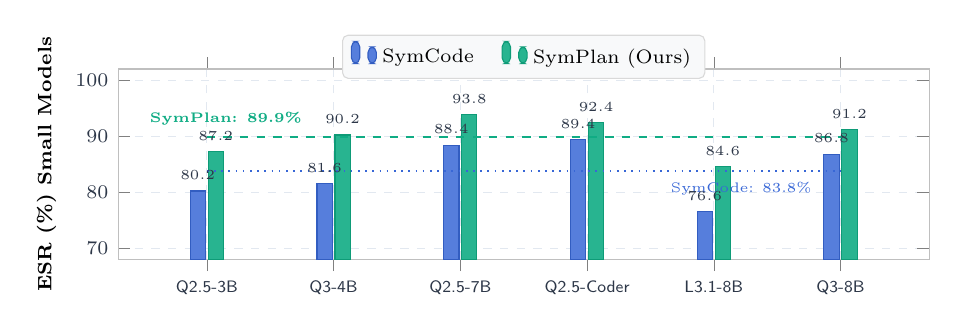
\begin{tikzpicture}
\begin{axis}[
    ybar=1.0pt,
    bar width=5.5pt,
    width=0.98\columnwidth,
    height=4.0cm,
    ymin=68,
    ymax=102,
    ytick={70, 80, 90, 100},
    ylabel={\scriptsize\textbf{ESR (\%) Small Models}},
    symbolic x coords={Q2.5-3B, Q3-4B, Q2.5-7B, Q2.5-Coder, L3.1-8B, Q3-8B},
    xtick=data,
    enlarge x limits=0.14,
    nodes near coords,
    nodes near coords style={font=\fontsize{4.2pt}{4.8pt}\selectfont\bfseries, text=chart_text, yshift=0.5pt},
    legend style={
        at={(0.5,1.18)},
        anchor=north,
        legend columns=2,
        font=\scriptsize,
        draw=gray!30,
        fill=boxgray,
        rounded corners=2pt,
        /tikz/every even column/.append style={column sep=8pt}
    },
    grid=major,
    grid style={draw=chart_grid, line width=0.4pt, dashed},
    axis line style={draw=gray!50},
    x tick label style={font=\fontsize{6pt}{7pt}\selectfont\sffamily, text=chart_text},
    y tick label style={font=\scriptsize\sffamily, text=chart_text}
]
\addplot[fill=color_symcode!85, draw=color_symcode!90!black, line width=0.4pt] coordinates {
    (Q2.5-3B, 80.20) (Q3-4B, 81.60) (Q2.5-7B, 88.40) (Q2.5-Coder, 89.40) (L3.1-8B, 76.60) (Q3-8B, 86.80)
};
\addplot[fill=color_symplan!90, draw=color_symplan!90!black, line width=0.4pt] coordinates {
    (Q2.5-3B, 87.20) (Q3-4B, 90.20) (Q2.5-7B, 93.80) (Q2.5-Coder, 92.40) (L3.1-8B, 84.60) (Q3-8B, 91.20)
};
\draw[dashed, color_symplan, line width=0.6pt] (axis cs:Q2.5-3B,89.90) -- (axis cs:Q3-8B,89.90) node[pos=0.03, above=0.5pt, font=\fontsize{4.5pt}{5.5pt}\selectfont\bfseries, text=color_symplan] {SymPlan: 89.9\%};
\draw[dotted, color_symcode, line width=0.6pt] (axis cs:Q2.5-3B,83.83) -- (axis cs:Q3-8B,83.83) node[pos=0.97, below=0.5pt, anchor=north east, font=\fontsize{4.5pt}{5.5pt}\selectfont, text=color_symcode] {SymCode: 83.8\%};
\legend{SymCode, SymPlan (Ours)}
\end{axis}
\end{tikzpicture}
\caption{Execution Success Rate (ESR \%) comparison between SymCode and SymPlan across all six models on MATH-500.}
\label{fig:chart}
\end{figure}

\subsection{Main Results}
\label{sec:results}

As shown in Table~\ref{tab:mainresults}, SymPlan delivers consistent accuracy gains across all six compact models, outperforming monolithic SymCode by $+3.60\%$ to $+5.20\%$ (averaging $+4.20\%$). The most pronounced improvements emerge on Qwen3-4B ($+5.20\%$) and Qwen2.5-Coder-7B ($+4.40\%$). Compared to natural-language CoT, SymPlan achieves an average improvement of $+12.64\%$ ($+23.20\%$ on Qwen2.5-Coder-7B and $+18.80\%$ on Qwen3-8B), confirming that symbolic solvers provide indispensable computational precision when guided by structured planning.

Furthermore, Fig.~\ref{fig:chart} illustrates that SymPlan increases average Execution Success Rate from $83.83\%$ to $89.90\%$ ($+6.07\%$), with notable gains on Llama-3.1-8B ($+8.00\%$) and Qwen3-4B ($+8.60\%$). By establishing explicit type contracts and exact SymPy rules upfront, SymPlan avoids undefined variables and syntax violations before code reaches the interpreter, reducing execution crashes by $37.5\%$.

In terms of inference cost, SymPlan incurs a moderate $22.6\%$ increase in tokens over SymCode ($392.9$ vs. $320.6$ tokens/problem across all models), dedicating $\approx 85$ tokens to the fused plan and $\approx 308$ tokens to code generation, while remaining more compact than natural-language CoT ($423.7$ tokens). This modest overhead prevents costly multi-round repair loops downstream.

\begin{table}[t]
\centering
\caption{Accuracy (\%) by difficulty level on MATH-500 for Qwen2.5-Coder-7B and Qwen3-8B.}
\label{tab:levels}
\resizebox{\columnwidth}{!}{%
\begin{tabular}{llcccc}
\toprule
\rowcolor{headergray}
\textbf{Model} & \textbf{Level (Count)} & \textbf{Direct} & \textbf{CoT} & \textbf{SymCode} & \textbf{SymPlan (Ours)} \\
\midrule
\multirow{5}{*}{Qwen2.5-Coder-7B} 
& Level 1 (43) & 41.86 & 88.37 & 88.37 & \textbf{88.37} \\
& Level 2 (90) & 36.67 & 64.44 & 74.44 & \textbf{83.33} \\
& Level 3 (105) & 26.67 & 46.67 & 61.90 & \textbf{73.33} \\
& Level 4 (128) & 12.50 & 27.34 & 49.22 & \textbf{50.00} \\
& Level 5 (134) & 11.19 & 8.21 & 38.81 & \textbf{39.55} \\
\midrule
\multirow{5}{*}{Qwen3-8B} 
& Level 1 (43) & 81.40 & 83.72 & 86.05 & \textbf{90.70} \\
& Level 2 (90) & 72.22 & 76.67 & 70.00 & \textbf{76.67} \\
& Level 3 (105) & 42.86 & 53.33 & 63.81 & \textbf{66.67} \\
& Level 4 (128) & 20.31 & 35.16 & 58.59 & \textbf{60.94} \\
& Level 5 (134) & 7.46 & 14.18 & 42.54 & \textbf{47.01} \\
\bottomrule
\end{tabular}}
\end{table}

\begin{table}[t]
\centering
\caption{Subject-wise accuracy (\%) on MATH-500 comparing CoT, SymCode (SC), and SymPlan (SP).}
\label{tab:subjects}
\resizebox{\columnwidth}{!}{%
\begin{tabular}{lccccccc}
\toprule
\rowcolor{headergray}
 & & \multicolumn{3}{c}{\textbf{Qwen2.5-Coder-7B}} & \multicolumn{3}{c}{\textbf{Qwen3-8B}} \\
\cmidrule(lr){3-5} \cmidrule(lr){6-8}
\rowcolor{headergray}
\textbf{Subject} & \textbf{Count} & \textbf{CoT} & \textbf{SC} & \textbf{SP} & \textbf{CoT} & \textbf{SC} & \textbf{SP} \\
\midrule
Algebra & 124 & 51.61 & 66.94 & \textbf{76.61} & 64.52 & 71.77 & \textbf{75.81} \\
Counting \& Prob. & 38 & 39.47 & 52.63 & \textbf{57.89} & 50.00 & 44.74 & \textbf{57.89} \\
Geometry & 41 & 36.59 & 31.71 & \textbf{34.15} & 39.02 & 46.34 & \textbf{51.22} \\
Interm. Algebra & 97 & 16.49 & \textbf{51.55} & 48.45 & 15.46 & 50.52 & \textbf{51.55} \\
Number Theory & 62 & 35.48 & 66.13 & \textbf{70.97} & 40.32 & 62.90 & \textbf{72.58} \\
Prealgebra & 82 & 62.20 & 69.51 & \textbf{75.61} & 73.17 & 73.17 & \textbf{73.17} \\
Precalculus & 56 & 14.29 & 37.50 & \textbf{41.07} & 17.86 & 46.43 & \textbf{48.21} \\
\bottomrule
\end{tabular}}
\end{table}

\subsection{Stratified Analysis by Difficulty and Subject}

Table~\ref{tab:levels} breaks down performance across difficulty tiers. On intermediate competition problems (Levels 2 and 3), SymPlan yields substantial double-digit gains over SymCode: on Qwen2.5-Coder-7B, accuracy rises from $74.44\%$ to $83.33\%$ on Level 2 ($+8.89\%$) and from $61.90\%$ to $73.33\%$ on Level 3 ($+11.43\%$). On challenging Level 5 problems, SymPlan maintains superior performance ($39.55\%$ vs. $38.81\%$ on Coder-7B; $47.01\%$ vs. $42.54\%$ on Qwen3-8B), markedly outperforming prose CoT ($8.21\%$ and $14.18\%$).

Table~\ref{tab:subjects} details subject-level performance. SymPlan achieves its largest gains in \textit{Algebra} ($+9.67\%$ on Coder-7B, $+4.04\%$ on Qwen3-8B), \textit{Counting \& Probability} ($+5.26\%$ and $+13.15\%$), and \textit{Number Theory} ($+4.84\%$ and $+9.68\%$). In these domains, implicit combinatorial and modular constraints are frequently omitted during monolithic generation; SymPlan's explicit contract $(\tau, \Omega)$ ensures these constraints are preserved in code. Note that the weighted averages across difficulty levels and subjects strictly reconstruct the overall benchmark accuracies in Table~\ref{tab:mainresults}.

\begin{figure}[t]
\centering
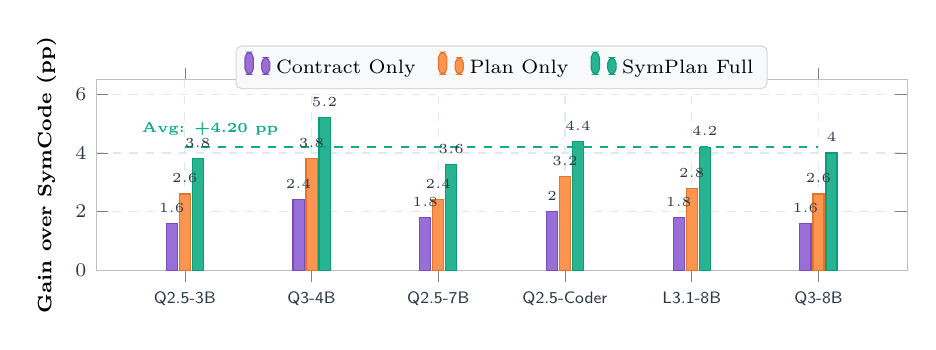
\begin{tikzpicture}
\begin{axis}[
    ybar=0.7pt,
    bar width=4.0pt,
    width=0.98\columnwidth,
    height=4.0cm,
    ymin=0,
    ymax=6.5,
    ytick={0, 2, 4, 6},
    ylabel={\scriptsize\textbf{Gain over SymCode (pp)}},
    symbolic x coords={Q2.5-3B, Q3-4B, Q2.5-7B, Q2.5-Coder, L3.1-8B, Q3-8B},
    xtick=data,
    enlarge x limits=0.14,
    grid=major,
    grid style={draw=chart_grid, line width=0.4pt, dashed},
    axis line style={draw=gray!50},
    x tick label style={font=\fontsize{6pt}{7pt}\selectfont\sffamily, text=chart_text},
    y tick label style={font=\scriptsize\sffamily, text=chart_text},
    nodes near coords,
    nodes near coords style={font=\fontsize{4.0pt}{4.5pt}\selectfont\bfseries, text=chart_text, yshift=0.5pt},
    legend style={
        at={(0.5,1.18)},
        anchor=north,
        legend columns=3,
        font=\scriptsize,
        draw=gray!30,
        fill=boxgray,
        rounded corners=2pt,
        /tikz/every even column/.append style={column sep=6pt}
    }
]
\addplot[fill=color_contract!85, draw=color_contract!90!black, line width=0.4pt] coordinates {
    (Q2.5-3B, 1.60) (Q3-4B, 2.40) (Q2.5-7B, 1.80) (Q2.5-Coder, 2.00) (L3.1-8B, 1.80) (Q3-8B, 1.60)
};
\addplot[fill=color_plan!85, draw=color_plan!90!black, line width=0.4pt] coordinates {
    (Q2.5-3B, 2.60) (Q3-4B, 3.80) (Q2.5-7B, 2.40) (Q2.5-Coder, 3.20) (L3.1-8B, 2.80) (Q3-8B, 2.60)
};
\addplot[fill=color_symplan!90, draw=color_symplan!90!black, line width=0.4pt] coordinates {
    (Q2.5-3B, 3.80) (Q3-4B, 5.20) (Q2.5-7B, 3.60) (Q2.5-Coder, 4.40) (L3.1-8B, 4.20) (Q3-8B, 4.00)
};
\draw[dashed, color_symplan, line width=0.6pt] (axis cs:Q2.5-3B,4.20) -- (axis cs:Q3-8B,4.20) node[pos=0.04, above=0.5pt, font=\fontsize{4.5pt}{5.5pt}\selectfont\bfseries, text=color_symplan] {Avg: +4.20 pp};
\legend{Contract Only, Plan Only, SymPlan Full}
\end{axis}
\end{tikzpicture}
\caption{Accuracy gains over SymCode (percentage points) in component ablation across all six models on MATH-500.}
\label{fig:ablation}
\end{figure}

\subsection{Component Ablation}
\label{sec:ablation}

To isolate the contributions of our framework, we evaluate three variants across all six models: (1) \textit{Contract-Only}, which enforces $(\tau, \Omega)$ without plan $\mathcal{P}$; (2) \textit{Plan-Only}, which uses plan $\mathcal{P}$ without type contract $\Omega$; and (3) \textit{Full SymPlan}. As shown in Fig.~\ref{fig:ablation}, both components independently improve upon monolithic SymCode, with planning providing the larger individual gain ($+2.40\%$ to $+3.80\%$). Combining contract-guided planning with anti-regression selection yields the highest accuracy across every model ($+3.60\%$ to $+5.20\%$).

\begin{table}[t]
\centering
\caption{Quantitative failure mode comparison between SymCode and SymPlan across all 3,000 problem evaluations on MATH-500.}
\label{tab:error_breakdown}
\resizebox{\columnwidth}{!}{%
\begin{tabular}{lcccc}
\toprule
\rowcolor{headergray}
\textbf{Failure Category} & \textbf{SymCode} & \textbf{SymPlan} & \textbf{Net Red.} & \textbf{Rel. Red.} \\
\midrule
Execution Failures (Syntax/Crash) & 485 (16.2\%) & 303 (10.1\%) & -182 & \textbf{-37.5\%} \\
Format / Type Mismatches & 515 (17.2\%) & 394 (13.1\%) & -121 & \textbf{-23.5\%} \\
Semantic Misformulations & 974 (32.5\%) & 969 (32.3\%) & -5 & -0.5\% \\
\midrule
\rowcolor{ourgreen}
\textbf{Total Incorrect Solutions} & 1489 (49.6\%) & 1363 (45.4\%) & -126 & \textbf{-8.5\%} \\
\bottomrule
\end{tabular}}
\end{table}

\subsection{Quantitative Error Diagnostics and Case Studies}
\label{sec:error_analysis}

Table~\ref{tab:error_breakdown} categorizes all failure cases across the 3,000 evaluations (6 models $\times$ 500 problems). SymPlan achieves a net reduction of 126 errors ($-8.5\%$ relative reduction), revealing distinct underlying mechanisms:

\textbf{1. Reduction in Execution Crashes (-37.5\%).} SymCode suffered 485 crashes ($16.2\%$) due to invalid syntax, non-existent library symbols, and runtime exceptions. SymPlan lowers crashes to 303 ($10.1\%$) by constraining code synthesis with standardized SymPy templates and exact rational rules.

\textbf{2. Mitigation of Format and Type Mismatches (-23.5\%).} Format mismatches dropped from 515 to 394 instances. Explicitly defining type contract $\Omega \in \{\texttt{number}, \texttt{text}, \texttt{tuple}, \texttt{set}, \texttt{symbolic}\}$ during fused planning directs models to output scalar cardinality rather than unrequested element sets.

\textbf{3. Preserving Structural Invariants.} For instance, on a degree-5 polynomial problem with $p(n) = n/(n^2 - 1)$ for $n \in \{2,\ldots,7\}$, monolithic SymCode produced an executable but disconnected polynomial and returned 39690 instead of $3/56$. The error was not numerical; SymCode failed to preserve the six interpolation constraints. SymPlan's representation explicitly registered the six exact point conditions, guiding the plan to apply Lagrange interpolation with rational arithmetic before evaluating $p(8)$.

\textbf{4. Boundaries of Structural Scaffolding.} Semantic misformulation remains largely unchanged ($974 \to 969$, a negligible $-0.5\%$ shift). This provides a key scientific insight: neurosymbolic scaffolding effectively resolves interface alignment and execution failures, but cannot compensate when a compact model fundamentally lacks the underlying mathematical concept (as on non-constructive Level-5 problems). Integrating interactive formal theorem provers (e.g., Lean) represents the natural next frontier for extreme non-constructive mathematics.

\section{Conclusion}

We presented SymPlan, an inspectable neurosymbolic framework tailored for mathematical problem solving in compact small language models. By decoupling monolithic generation into a fused target-planning phase, contract-guided SymPy code synthesis, and targeted debugging with anti-regression ranking, SymPlan mitigates semantic misformulation, domain omission, and repair regressions. Across six diverse compact models (3B--8B) on the full MATH-500 benchmark under 4-bit quantization, SymPlan achieves uniform accuracy gains of $+3.60\%$ to $+5.20\%$ over SymCode and up to $+23.20\%$ over CoT, while improving Execution Success Rate to $89.90\%$, all without parameter updates. In future work, we plan to extend SymPlan to multimodal geometric diagrams and integrate formal proof verifiers on edge devices.

\IEEEtriggeratref{19}
\bibliographystyle{IEEEtran}
\bibliography{cite}

\end{document}
